Se presentará a continuación un breve manual de usuario sobre la Filter Tool implementada para el presente
trabajo práctico.

\subsection{Etapa 1}

A continuación se puede ver la pantalla general de la Etapa 1:

\begin{figure}[H]
    \centering
    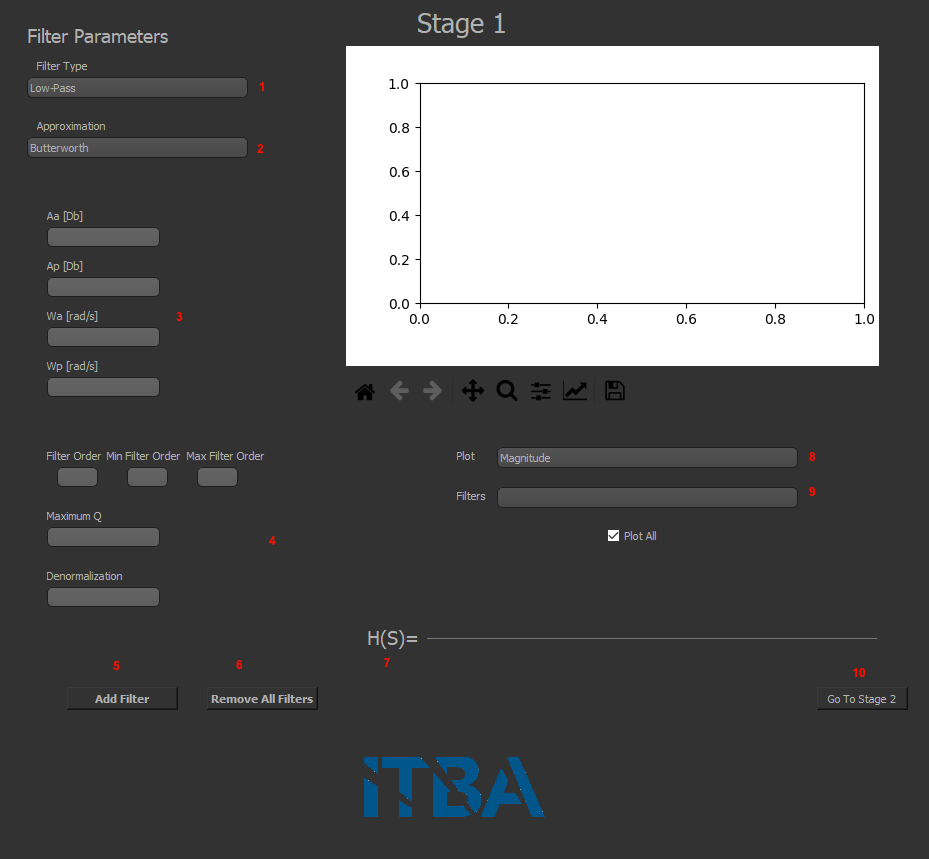
\includegraphics[width=0.85\textwidth]{../Ejercicio1-FilterTool/Imagenes/imagen-general-1.png}
    \caption{Etapa 1 - Vista General}
    \label{ImagenGeneral}
\end{figure}

\subsubsection{Tipos de Filtro}

Se podrán realizar los siguientes tipos de filtro con la herramiento diseñada:

\begin{itemize}
	\item Low-Pass
	\item High-Pass
	\item Band-Pass
	\item Band-Rejection
	\item Group-Delay
\end{itemize}

Ellos pueden ser seleccionados desplegando el selector ubicado en $1$ que se puede observar en la figura $\ref{ImagenGeneral}$.
Es importante destacar que durante la implementación final del trabajo práctico, Group-Delay no pudo ser implementado en su totalidad por una cuestión de tiempo.
Para ello, se intentó utilizar la aproximación de Gauss. De todas formas, el código desarrollado se encuentra en el archivo $gauss.py$ pero en la versión final
de la herramienta puede sufrir comportamientos inesperados o no calcular un filtro mediante esta aproximación. 

El resto de los tipos de filtros pueden ser empleados en su totalidad con solo el hecho de seleccionarlos.

\subsubsection{Tipos de Aproximación}

Se pueden elegir entre los siguientes tipos de aproximación para calcular los tipos de filtro mencionados precedentemente:

\begin{itemize}
	\item Butterworth
	\item Cauer
	\item Chebychev 1
	\item Chebychev 2
	\item Legendre
\end{itemize}

Ellos podrán ser utilizados para cualquiera de los tipos de filtro y se podrán seleccionar desde $2$ de la figura $\ref{ImagenGeneral}$.

\subsubsection{Parámetros de Plantilla}

En $3$ de la figura $\ref{ImagenGeneral}$ se podrán ingresar los parámetros de la plantilla que deberá cumplir el filtro a crear.
Dependiendo si es un filtro Low-Pass, High-Pass o Band-Pass, Band-Rejection, se desplegarán los parámetros necesarios para que la 
aplicación pueda crear el filtro.

Los valores se ingresarán por teclado y se podrán ingresar valores en notación científica, expresados como en el siguiente ejemplo:

$$100e3 \Longrightarrow 100000$$

Dichos valores podrán ser modificados cuantas veces sea necesario previo a crear el filtro. Dependiendo el tipo de filtro,
todos estos valores deben ser ingresados por el usuario obligatoriamente.

\begin{figure}[H]
    \centering
    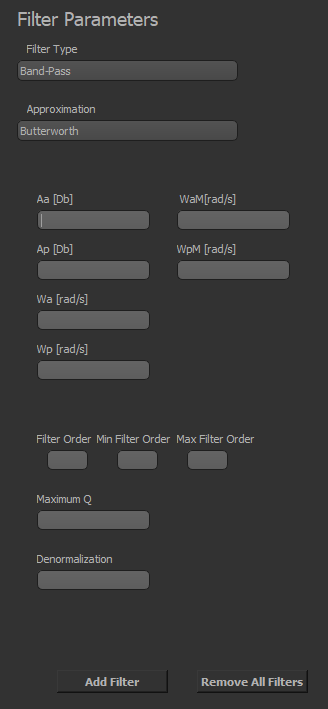
\includegraphics[scale=0.5]{../Ejercicio1-FilterTool/Imagenes/opciones.png}
    \caption{Ejemplo de Parámetros de plantilla para un filtro BP o BR}
\end{figure}

\subsubsection{Parámetros de Filtro}

En $4$ de la figura $\ref{ImagenGeneral}$ se ingresarán los parámetros del filtro en cuestión. Ellos no son obligatorios, ya que en el caso de ser omitidos
tomarán valores por defecto.

\begin{itemize}
	\item Filter Order: Si no se especifica, el filtro se diseñará sin limitaciones. Caso contrario, se diseñará un filtro que tenga dicho orden.
	\item Min Filter Order: Si no se especifica, el filtro se diseñará sin limitaciones. Caso contrario, el filtro cumplirá mínimamente este orden.
	\item Max Filter Order: Si no se especifica, el filtro se diseñará con un orden máximo de 10. Caso contrario, el filtro tendrá como mucho dicho orden.
	\item Maximum Q: Si no se especifica, el filtro se diseñará sin limitaciones. Caso contrario, el filtro no superará dicho Q.
	\item Denormalization: Si no se especifica, el filtro se diseñará con una denormalización de 0. Puede tomar un valor máximo de 1.
\end{itemize}

Se podrán modificar cuantas veces sea necesario, previo a añadir un nuevo filtro. Es importante destacar que por una cuestión de diseño el orden máximo de un filtro posible es de 10.

\subsubsection{Agregar Filtro}

Una vez completados mínimamente los parámetros obligatorios, se podrá añadir un nuevo filtro, seleccionado $5$ de la figura $\ref{ImagenGeneral}$. La aplicación validará
que los parámetros ingresados son pertinentes para el tipo de filtro y la aproximación deseada. En el caso de que los parámetros sean incorrectos, la aplicación emitirá
una alerta indicando que parámetros son los incorrectos para ser remediados.

Se podrán añadir tantos filtros como se deseen, siempre y cuando no se cambien los parámetros ingresados en $4$ o el tipo de filtro, es decir que no se cambie la plantilla.
En el caso de que se añada un filtro con una plantilla diferente se podrá escoger borrar los anteriores con una plantilla diferente, o editar el filtro a ingresar
para que conserve la misma.

En resumen, siempre que se mantengan el tipo de filtro y los valores de plantilla, se añadirán la cantidad necesaria de filtros.
Ello además para observar comparativamente el comportamiento de las distintas aproximaciones para un mismo tipo de filtro.

\subsubsection{Remover todos los filtros}

Seleccionando $6$ se podrán remover todos los filtros añadidos previamente. Ello implicará que el usuario podrá empezar nuevamente
como si estuviese iniciando la aplicación. Esta acción no se puede deshacer.

\subsubsection{Función Transferencia}

En $7$ se podrá observar la función transferencia $H(S)$ para el filtro añadido y seleccionado.

\subsubsection{Tipo de Plot}

En $8$ se podrá elegir qué tipo de gráfico se desea obtener para un filtro añadido o todos los filtros añadidos.
Con dicha herramienta se podrá comparar u observar el comportamiento individual de cada filtro en los siguientes gráficos:

\begin{itemize}
	\item Respuesta en Frecuencia - Magnitud
	\item Respuesta en Frecuencia - Fase
	\item Polos y ceros
	\item Retardo de Grupo
	\item Atenuación
	\item Atenuación Normalizada Low-Pass
	\item Respuesta al Impulso
	\item Respuesta al Escalón
\end{itemize}

Para todos los gráficos se podrá observar el comportamiento de un filtro en cuestión, variando el selector en $9$ en donde 
se irá añadiendo cada filtro ingresado por el usuario con una identificación que cuenta con el tipo de filtro, orden, aproximación
utilizada y denormalización.

Si se selecciona $Plot$ $All$, se observarán todos los filtros para el tipo de plot elegido. Si no se selecciona,
se podrá ver e iterar en cada filtro seleccionado mediante $Filters$ para observar el comportamiento individual.

A continuación se puede ver un ejemplo de respuesta en frecuencia (amplitud) para varios filtros Low-Pass.
\begin{figure}[H]
    \centering
    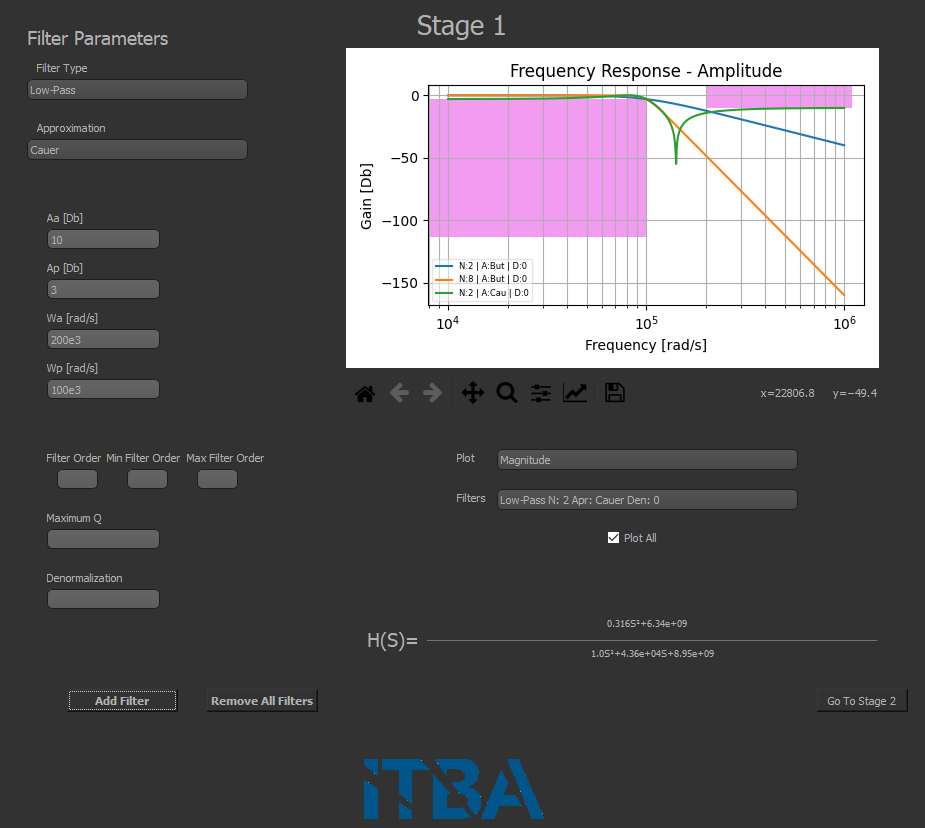
\includegraphics[width=0.85\textwidth]{../Ejercicio1-FilterTool/Imagenes/imagen-general-2-varias funciones.png}
    \caption{Etapa 1 - Ejemplo de Plot con Varios Filtros}
    \label{ImagenGeneralVariosFiltros}
\end{figure}

La función transferencia visible en pantalla será siempre la del filtro que esté seleccionado en $Filters$.

\subsubsection{Filtros Diseñados}

En $9$ se añadirán automáticamente todos los filtros creados para poder trabajar con ellos y seleccionarlos para obtener
el gráfico o función transferencia deseada.

\subsubsection{Ir a Etapa 2}

Si se cuenta mínimamente con un filtro añadido, se podrá proceder a la etapa 2, seleccionado $10$ 
de la figura $\ref{ImagenGeneral}$.

En dicha etapa se trabajará sobre un filtro únicamente. Para seleccionar qué filtro de los diseñados será
el elegido para proceder a la etapa 2, bastará con seleccionarlo en el seleccionador de filtros $Filters$. Es importante saber que al pasar a la Etapa 2 con un filtro seleccionado, no implicará que todos los filtros de la Etapa 1 sean eliminados.
Ellos seguirán estando disponibles siempre y cuando se vuelva a la etapa 1. 

\subsection{Etapa 2}

Una vez escogido el filtro diseñado en la etapa 1, luego de haber analizado su comportamiento utilizando los distintos
tipos de gráficos y función de transferencia, se procede a trabajar sobre él en la etapa 2, haciendo los ajustes que el usuario considere necesarios.

\begin{figure}[H]
    \centering
    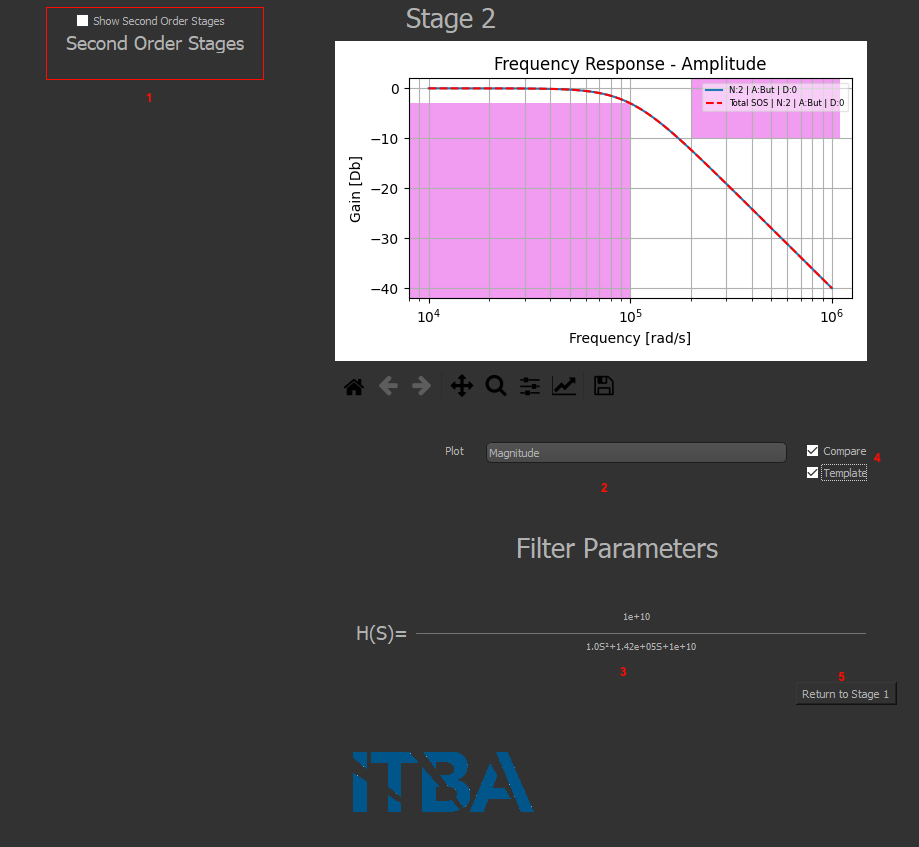
\includegraphics[width=0.85\textwidth]{../Ejercicio1-FilterTool/Imagenes/con-plantilla.png}
    \caption{Etapa 2 - Vista General}
    \label{Etapa2}
\end{figure}

\subsubsection{Trabajar con etapas de Segundo y Primer Orden}

Si el usuario selecciona $Show$ $Second$ $Order$ $Stages$, que se puede observar en $1$
de la figura \ref{Etapa2}, se mostrarán sistemas de segundo y primer orden que en su conjunto
conforman al filtro total diseñado.

Obviamente si el orden de los filtros es impar, se empleará un filtro de primer orden y el resto de segundo orden.
Si el orden es par, todas las etapas serán de segundo orden. Es importante notar que para el diseño de cada etapa,
se planteó en el código desarrollado que la ganancia del filtro total se distribuya equitativamente. Ese es el comportamiento default, aunque para un desarrollo posterior,
se puede cambiar la variable $DistribuiteGainBetweenAllSections$ a un valor de $False$ y la ganancia será absorbida por la última etapa.

A continuación se puede ver el comportamiento de dicha funcionalidad para un sistema de octavo orden de tipo Low-Pass.

\begin{figure}[H]
    \centering
    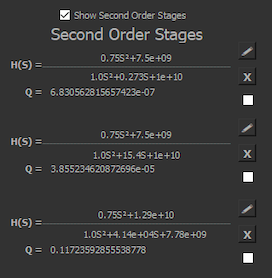
\includegraphics[scale=0.5]{../Ejercicio1-FilterTool/Imagenes/SOS.png}
    \caption{Etapa 2 - Sistemas de Segundo Orden}
\end{figure}

Se puede ver que para cada etapa, la herramienta mostrará su función transferencia así como su Q.

A su vez, se podrá editar cada uno de ellas o removerla del circuito total. Para editar una etapa en particular basta con seleccionar el símbolo del $lapiz$ para cada una de ellas. Se podrá cambiar la función transferencia de dicha etapa,
por ende modificarla en su totalidad incluyendo la ganancia. Con el botón "X" se podrá remover dicha etapa.

Para editar una etapa en particular, una vez seleccionada la acción de Editar, se deberá ingresar la función transferencia en formato numerador y denominador:

$$H(S) = \frac{aS^n + bS^{n-1}+ ... +cS^{n-i}}{eS^m + fS^{m-1}+ ... +gS^{m-j}} $$

Para ello, se deben completar los campos correspondientes ingresando los valores de los coeficientes del polinomio del numerador y denominador correspondientemente separados por ",". El primer valor ingresado tanto para el numerador como el denominador representarán el coeficiente de la potencia de mayor grado del polinomio y los siguientes elementos representarán los de grado $n-1, n -2 , ... , n-m$. 
Deberán ingresarse tantos elementos como coeficientes haya en el polinomio que se quiera representar. En los casos donde haya coeficientes nulos, se deberán ingresar $0$ como elemento.
En caso de que se deseen representar coeficientes que no sean números enteros, podrá utilizarse $"."$ .
Es decir, que si queremos representar un polinomio de grado $n$ y algunos o todos los coeficientes de las potencias de grado menor son nulas, indefectiblemente, el usuario deberá ingresar $0$ para poder alcanzar el grado deseado del polinomio.

Una vez ingresados y aceptados los parámetros dicha etapa será reemplazada por la editada individualmente.

A continuación se puede ver como se puede editar dicha etapa:

\begin{figure}[H]
    \centering
    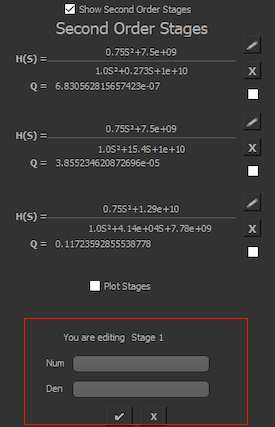
\includegraphics[scale=0.5]{../Ejercicio1-FilterTool/Imagenes/sosEdit.png}
    \caption{Etapa 2 - Sistemas de Segundo Orden}
\end{figure}

Siempre la función diseñada en la etapa 1 quedará guardada y visible en la etapa 2 para que el usuario pueda comparar su comportamiento a medida
que se editan las etapas individualmente o se remueven. Cada cambio realizado sobre el filtro permanecerá en la etapa 2, a menos que se vuelva a la etapa 1.

\subsubsection{Tipo de Plot}

En $2$ de la figura \ref{Etapa2}, se podrá elegir qué tipo de gráfico se podrá observar para el filtro en cuestión. Los tipos de gráfico para esta etapa son:


\begin{itemize}
	\item Respuesta en Frecuencia - Magnitud
	\item Respuesta en Frecuencia - Fase
	\item Polos y Ceros
\end{itemize}

En $4$ de la figura \ref{Etapa2}, se contará con dos checkbox para la respuesta en frecuencia (magnitud):

\begin{itemize}
	\item Compare: Si está seleccionado, se mostrará en el gráfico tanto la función del filtro original obtenido en la Etapa 1 como el filtro resultante a medida que se va editando cada etapa.
	\item Template: Para observar si el filtro editado por etapas cumple la plantilla seleccionada en la Etapa 1, se podrá observar o no la plantilla en el gráfico.
\end{itemize}

Si el gráfico seleccionado es respuesta en frecuencia (Fase), solo se observará la opción $Compare$ obteniendo el mismo efecto que para el gráfico de respuesta en frecuencia (magnitud).

Finalmente para el gráfico de Polos y Ceros, solo se observarán los de la función original. A continuación se puede ver un caso donde el usuario removió una etapa de un filtro diseñado y su comparación gráfica utilizando a su vez la plantilla.

\begin{figure}[H]
    \centering
    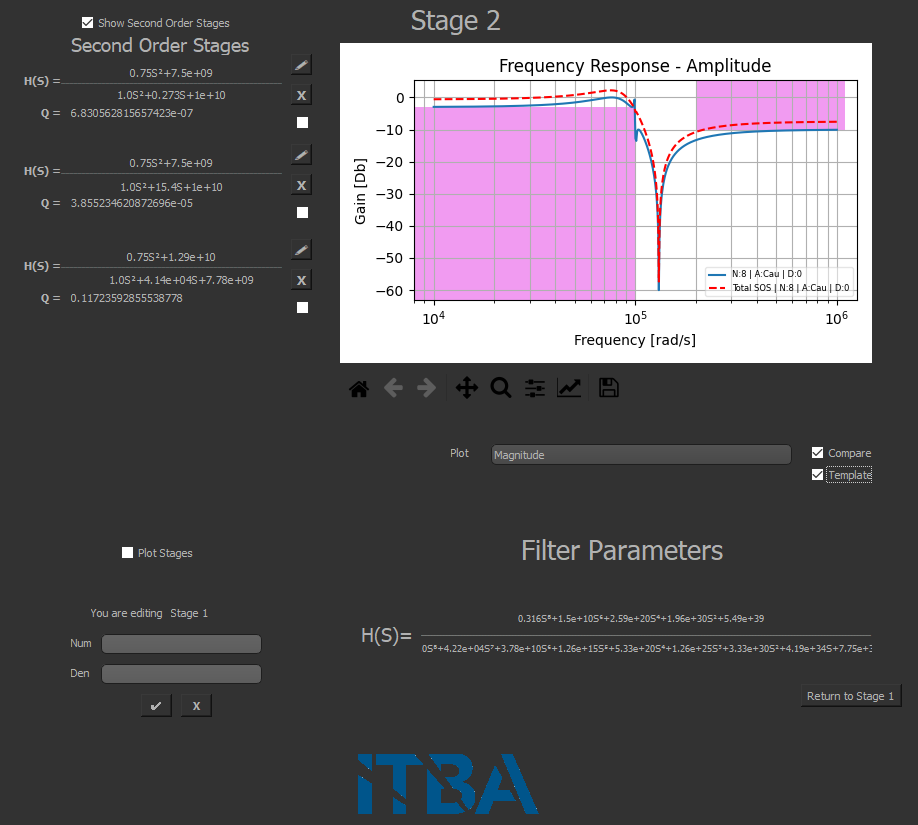
\includegraphics[width=0.85\textwidth]{../Ejercicio1-FilterTool/Imagenes/comparame-com-plantilla.png}
    \caption{Etapa 2 - Ejemplo de Plot con Filtro Original y Editado}
\end{figure}

En la siguiente figura, se puede observar un gráfico comparativo donde el usuario no realizó ninguna modificación:

\begin{figure}[H]
    \centering
    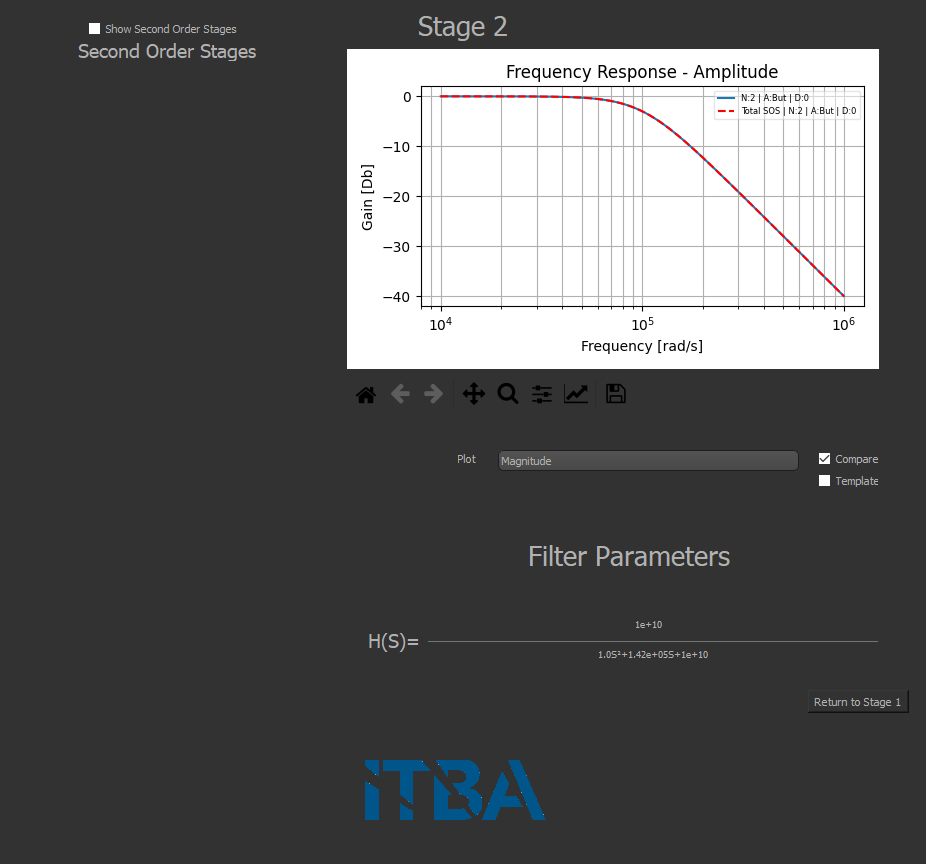
\includegraphics[width=0.85\textwidth]{../Ejercicio1-FilterTool/Imagenes/comparacion.png}
    \caption{Etapa 2 - Ejemplo de Plot con Filtro Original y Representado por Etapas}
\end{figure}

El filtro que se está editando será identificado con "SOS" en los labels de cada gráfico.

\subsubsection{Tipo de Plot - Etapas individuales}

Si se selecciona $Plot$ $Stages$ en la pantalla donde se encuentran los sistemas de segundo orden, se podrá obtener gráficamete la respuesta en frecuencia (amplitud y fase) para cada etapa, alguna de ellas o todas.

Para cada etapa que se desee obtener su gráfico bastará con seleccionarla con el checkbox debajo de "X". Ello hará que se la incluya dentro de los gráficos o non. Para volver al modo anterior donde se puede comparar el filtro total con el filtro total editado,
bastará con no seleccionar $Plot$ $Stage$.

\begin{figure}[H]
    \centering
    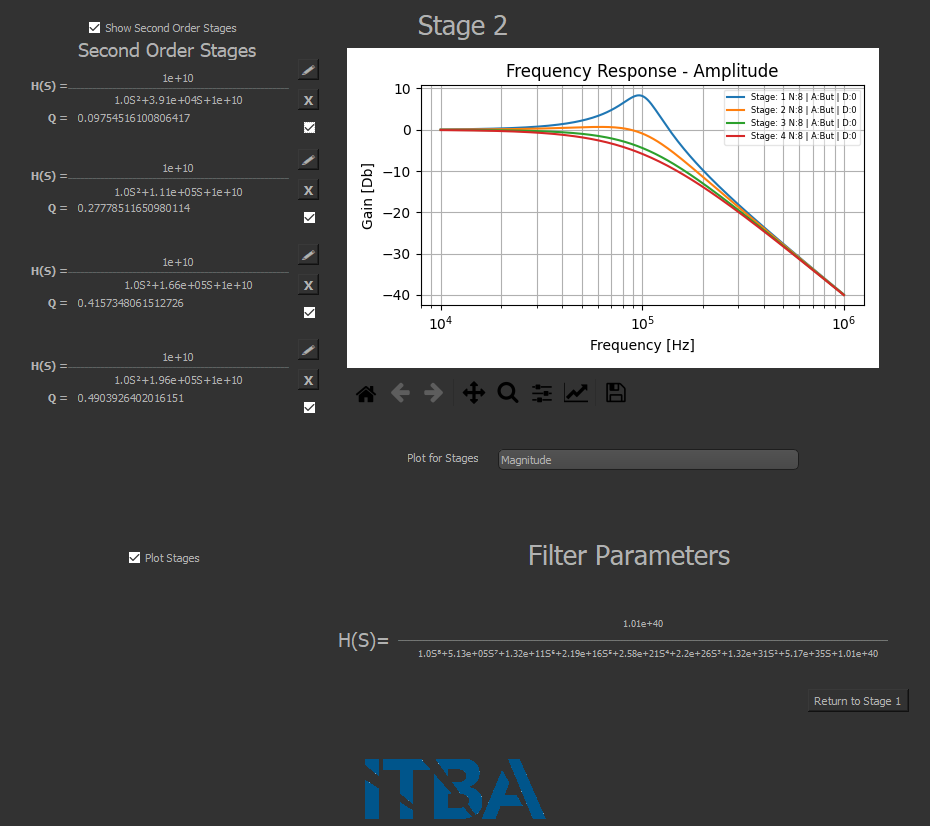
\includegraphics[width=0.85\textwidth]{../Ejercicio1-FilterTool/Imagenes/stage-plot.png}
    \caption{Etapa 2 - Ploteo de cada Etapa de Segundo Orden}
\end{figure}

\subsection{Resumen de Workflow de Diseño}

\begin{itemize}
	\item El usuario podrá elegir algún tipo de filtro de los mencionados previamente, y establecer una plantilla que deba cumplir.
	\item Estableciendo parámetros del filtro como el orden, la aproximación, el Q o la denormalización, se podrán agregar tantos filtros como se desee para observar su comportamiento y elegir el más adecuado.
	\item Se podrán observar múltiples gráficos de interés para comparar el comportamiento del filtro ya sea de manera comparativa o individual.
	\item Una vez seleccionado el filtro, se podrá proceder a la Etapa 2, donde el usuario podrá trabajar en etapas de segundo y primer orden y editar cada una de ellas individualmente que conformarán al filtro total.
	\item El hecho de editar cada etapa implica que se la podrá remover o editar en su totalidad.
	\item Al editar cada etapa se podrá observar comparativamente el filtro original obtenido en la Etapa 1 y el resultante luego de aplicar cambios sobre cada etapa.
	\item Finalmente como último análisis se podrá obtener la respuesta en frecuencia para cada etapa para observar que su comportamiento no tenga efectos adversos individualmente.
	\item Si el usuario lo desea, podrá volver a la etapa 1, perdiendo todos los cambios realizados en la etapa 2, pero con los filtros diseñados previamente disponibles. 
\end{itemize}

